\documentclass[1p]{elsarticle_modified}
%\bibliographystyle{elsarticle-num}

%\usepackage[colorlinks]{hyperref}
%\usepackage{abbrmath_seonhwa} %\Abb, \Ascr, \Acal ,\Abf, \Afrak
\usepackage{amsfonts}
\usepackage{amssymb}
\usepackage{amsmath}
\usepackage{amsthm}
\usepackage{scalefnt}
\usepackage{amsbsy}
\usepackage{kotex}
\usepackage{caption}
\usepackage{subfig}
\usepackage{color}
\usepackage{graphicx}
\usepackage{xcolor} %% white, black, red, green, blue, cyan, magenta, yellow
\usepackage{float}
\usepackage{setspace}
\usepackage{hyperref}

\usepackage{tikz}
\usetikzlibrary{arrows}

\usepackage{multirow}
\usepackage{array} % fixed length table
\usepackage{hhline}

%%%%%%%%%%%%%%%%%%%%%
\makeatletter
\renewcommand*\env@matrix[1][\arraystretch]{%
	\edef\arraystretch{#1}%
	\hskip -\arraycolsep
	\let\@ifnextchar\new@ifnextchar
	\array{*\c@MaxMatrixCols c}}
\makeatother %https://tex.stackexchange.com/questions/14071/how-can-i-increase-the-line-spacing-in-a-matrix
%%%%%%%%%%%%%%%

\usepackage[normalem]{ulem}

\newcommand{\msout}[1]{\ifmmode\text{\sout{\ensuremath{#1}}}\else\sout{#1}\fi}
%SOURCE: \msout is \stkout macro in https://tex.stackexchange.com/questions/20609/strikeout-in-math-mode

\newcommand{\cancel}[1]{
	\ifmmode
	{\color{red}\msout{#1}}
	\else
	{\color{red}\sout{#1}}
	\fi
}

\newcommand{\add}[1]{
	{\color{blue}\uwave{#1}}
}

\newcommand{\replace}[2]{
	\ifmmode
	{\color{red}\msout{#1}}{\color{blue}\uwave{#2}}
	\else
	{\color{red}\sout{#1}}{\color{blue}\uwave{#2}}
	\fi
}

\newcommand{\Sol}{\mathcal{S}} %segment
\newcommand{\D}{D} %diagram
\newcommand{\A}{\mathcal{A}} %arc


%%%%%%%%%%%%%%%%%%%%%%%%%%%%%5 test

\def\sl{\operatorname{\textup{SL}}(2,\Cbb)}
\def\psl{\operatorname{\textup{PSL}}(2,\Cbb)}
\def\quan{\mkern 1mu \triangleright \mkern 1mu}

\theoremstyle{definition}
\newtheorem{thm}{Theorem}[section]
\newtheorem{prop}[thm]{Proposition}
\newtheorem{lem}[thm]{Lemma}
\newtheorem{ques}[thm]{Question}
\newtheorem{cor}[thm]{Corollary}
\newtheorem{defn}[thm]{Definition}
\newtheorem{exam}[thm]{Example}
\newtheorem{rmk}[thm]{Remark}
\newtheorem{alg}[thm]{Algorithm}

\newcommand{\I}{\sqrt{-1}}
\begin{document}

%\begin{frontmatter}
%
%\title{Boundary parabolic representations of knots up to 8 crossings}
%
%%% Group authors per affiliation:
%\author{Yunhi Cho} 
%\address{Department of Mathematics, University of Seoul, Seoul, Korea}
%\ead{yhcho@uos.ac.kr}
%
%
%\author{Seonhwa Kim} %\fnref{s_kim}}
%\address{Center for Geometry and Physics, Institute for Basic Science, Pohang, 37673, Korea}
%\ead{ryeona17@ibs.re.kr}
%
%\author{Hyuk Kim}
%\address{Department of Mathematical Sciences, Seoul National University, Seoul 08826, Korea}
%\ead{hyukkim@snu.ac.kr}
%
%\author{Seokbeom Yoon}
%\address{Department of Mathematical Sciences, Seoul National University, Seoul, 08826,  Korea}
%\ead{sbyoon15@snu.ac.kr}
%
%\begin{abstract}
%We find all boundary parabolic representation of knots up to 8 crossings.
%
%\end{abstract}
%\begin{keyword}
%    \MSC[2010] 57M25 
%\end{keyword}
%
%\end{frontmatter}

%\linenumbers
%\tableofcontents
%
\newcommand\colored[1]{\textcolor{white}{\rule[-0.35ex]{0.8em}{1.4ex}}\kern-0.8em\color{red} #1}%
%\newcommand\colored[1]{\textcolor{white}{ #1}\kern-2.17ex	\textcolor{white}{ #1}\kern-1.81ex	\textcolor{white}{ #1}\kern-2.15ex\color{red}#1	}

{\Large $\underline{10_{65}~(K10a_{42})}$}

\setlength{\tabcolsep}{10pt}
\renewcommand{\arraystretch}{1.6}
\vspace{1cm}\begin{tabular}{m{100pt}>{\centering\arraybackslash}m{274pt}}
\multirow{5}{120pt}{
	\centering
	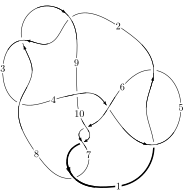
\includegraphics[width=112pt]{../../../GIT/diagram.site/Diagrams/png/149_10_65.png}\\
\ \ \ A knot diagram\footnotemark}&
\allowdisplaybreaks
\textbf{Linearized knot diagam} \\
\cline{2-2}
 &
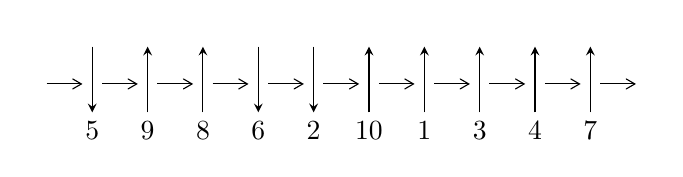
\begin{tikzpicture}[x=20pt, y=17pt]
	% nodes
	\node (C0) at (0, 0) {};
	\node (C1) at (1, 0) {};
	\node (C1U) at (1, +1) {};
	\node (C1D) at (1, -1) {5};

	\node (C2) at (2, 0) {};
	\node (C2U) at (2, +1) {};
	\node (C2D) at (2, -1) {9};

	\node (C3) at (3, 0) {};
	\node (C3U) at (3, +1) {};
	\node (C3D) at (3, -1) {8};

	\node (C4) at (4, 0) {};
	\node (C4U) at (4, +1) {};
	\node (C4D) at (4, -1) {6};

	\node (C5) at (5, 0) {};
	\node (C5U) at (5, +1) {};
	\node (C5D) at (5, -1) {2};

	\node (C6) at (6, 0) {};
	\node (C6U) at (6, +1) {};
	\node (C6D) at (6, -1) {10};

	\node (C7) at (7, 0) {};
	\node (C7U) at (7, +1) {};
	\node (C7D) at (7, -1) {1};

	\node (C8) at (8, 0) {};
	\node (C8U) at (8, +1) {};
	\node (C8D) at (8, -1) {3};

	\node (C9) at (9, 0) {};
	\node (C9U) at (9, +1) {};
	\node (C9D) at (9, -1) {4};

	\node (C10) at (10, 0) {};
	\node (C10U) at (10, +1) {};
	\node (C10D) at (10, -1) {7};
	\node (C11) at (11, 0) {};

	% arrows
	\draw[->,>={angle 60}]
	(C0) edge (C1) (C1) edge (C2) (C2) edge (C3) (C3) edge (C4) (C4) edge (C5) (C5) edge (C6) (C6) edge (C7) (C7) edge (C8) (C8) edge (C9) (C9) edge (C10) (C10) edge (C11) ;	\draw[->,>=stealth]
	(C1U) edge (C1D) (C2D) edge (C2U) (C3D) edge (C3U) (C4U) edge (C4D) (C5U) edge (C5D) (C6D) edge (C6U) (C7D) edge (C7U) (C8D) edge (C8U) (C9D) edge (C9U) (C10D) edge (C10U) ;
	\end{tikzpicture} \\
\hhline{~~} \\& 
\textbf{Solving Sequence} \\ \cline{2-2} 
 &
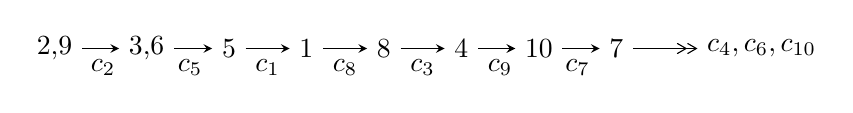
\begin{tikzpicture}[x=28pt, y=7pt]
	% node
	\node (A0) at (-1/8, 0) {2,9};
	\node (A1) at (17/16, 0) {3,6};
	\node (A2) at (17/8, 0) {5};
	\node (A3) at (25/8, 0) {1};
	\node (A4) at (33/8, 0) {8};
	\node (A5) at (41/8, 0) {4};
	\node (A6) at (49/8, 0) {10};
	\node (A7) at (57/8, 0) {7};
	\node (C1) at (1/2, -1) {$c_{2}$};
	\node (C2) at (13/8, -1) {$c_{5}$};
	\node (C3) at (21/8, -1) {$c_{1}$};
	\node (C4) at (29/8, -1) {$c_{8}$};
	\node (C5) at (37/8, -1) {$c_{3}$};
	\node (C6) at (45/8, -1) {$c_{9}$};
	\node (C7) at (53/8, -1) {$c_{7}$};
	\node (A8) at (9, 0) {$c_{4},c_{6},c_{10}$};

	% edge
	\draw[->,>=stealth]	
	(A0) edge (A1) (A1) edge (A2) (A2) edge (A3) (A3) edge (A4) (A4) edge (A5) (A5) edge (A6) (A6) edge (A7) ;
	\draw[->>,>={angle 60}]	
	(A7) edge (A8);
\end{tikzpicture} \\ 

\end{tabular} \\

\footnotetext{
The image of knot diagram is generated by the software ``\textbf{Draw programme}" developed by Andrew Bartholomew(\url{http://www.layer8.co.uk/maths/draw/index.htm\#Running-draw}), where we modified some parts for our purpose(\url{https://github.com/CATsTAILs/LinksPainter}).
}\phantom \\ \newline 
\centering \textbf{Ideals for irreducible components\footnotemark of $X_{\text{par}}$} 
 
\begin{align*}
I^u_{1}&=\langle 
-2 u^{24}+2 u^{23}+\cdots+4 b+2,\;2 u^{24}- u^{23}+\cdots+4 a-6,\;u^{25}-2 u^{24}+\cdots-4 u+2\rangle \\
I^u_{2}&=\langle 
- a^2 u^2+u^2 a+2 a u+b+2 a+2 u,\;-2 a^2 u^2+a^3+2 u^2 a-2 a^2+3 a u+5 a+u+1,\;u^3+u^2+2 u+1\rangle \\
I^u_{3}&=\langle 
b+1,\;2 a+u+2,\;u^2+2\rangle \\
\\
I^v_{1}&=\langle 
a,\;b-1,\;v-1\rangle \\
\end{align*}
\raggedright * 4 irreducible components of $\dim_{\mathbb{C}}=0$, with total 37 representations.\\
\footnotetext{All coefficients of polynomials are rational numbers. But the coefficients are sometimes approximated in decimal forms when there is not enough margin.}
\newpage
\renewcommand{\arraystretch}{1}
\centering \section*{I. $I^u_{1}= \langle -2 u^{24}+2 u^{23}+\cdots+4 b+2,\;2 u^{24}- u^{23}+\cdots+4 a-6,\;u^{25}-2 u^{24}+\cdots-4 u+2 \rangle$}
\flushleft \textbf{(i) Arc colorings}\\
\begin{tabular}{m{7pt} m{180pt} m{7pt} m{180pt} }
\flushright $a_{2}=$&$\begin{pmatrix}1\\0\end{pmatrix}$ \\
\flushright $a_{9}=$&$\begin{pmatrix}0\\u\end{pmatrix}$ \\
\flushright $a_{3}=$&$\begin{pmatrix}1\\- u^2\end{pmatrix}$ \\
\flushright $a_{6}=$&$\begin{pmatrix}-\frac{1}{2} u^{24}+\frac{1}{4} u^{23}+\cdots-2 u+\frac{3}{2}\\\frac{1}{2} u^{24}-\frac{1}{2} u^{23}+\cdots+\frac{3}{2} u-\frac{1}{2}\end{pmatrix}$ \\
\flushright $a_{5}=$&$\begin{pmatrix}-\frac{1}{4} u^{23}-\frac{5}{2} u^{21}+\cdots-\frac{1}{2} u+1\\\frac{1}{2} u^{24}-\frac{1}{2} u^{23}+\cdots+\frac{3}{2} u-\frac{1}{2}\end{pmatrix}$ \\
\flushright $a_{1}=$&$\begin{pmatrix}-\frac{1}{2} u^{24}+u^{23}+\cdots-3 u+\frac{3}{2}\\\frac{1}{4} u^{22}-\frac{1}{4} u^{21}+\cdots-\frac{1}{2} u-1\end{pmatrix}$ \\
\flushright $a_{8}=$&$\begin{pmatrix}- u\\u^3+u\end{pmatrix}$ \\
\flushright $a_{4}=$&$\begin{pmatrix}u^2+1\\- u^4-2 u^2\end{pmatrix}$ \\
\flushright $a_{10}=$&$\begin{pmatrix}u^5+2 u^3+u\\- u^7-3 u^5-2 u^3+u\end{pmatrix}$ \\
\flushright $a_{7}=$&$\begin{pmatrix}\frac{1}{4} u^{18}+2 u^{16}+\cdots-\frac{3}{2} u+\frac{1}{2}\\\frac{1}{2} u^{11}+\frac{5}{2} u^9+\cdots- u^2+u\end{pmatrix}$\\&\end{tabular}
\flushleft \textbf{(ii) Obstruction class $= -1$}\\~\\
\flushleft \textbf{(iii) Cusp Shapes $= -2 u^{24}+4 u^{23}-26 u^{22}+40 u^{21}-138 u^{20}+164 u^{19}-384 u^{18}+346 u^{17}-584 u^{16}+380 u^{15}-430 u^{14}+186 u^{13}-50 u^{12}+32 u^{11}+80 u^{10}+56 u^9-74 u^8+110 u^7-178 u^6+100 u^5-82 u^4+18 u^3+24 u^2-14 u+8$}\\~\\
\newpage\renewcommand{\arraystretch}{1}
\flushleft \textbf{(iv) u-Polynomials at the component}\newline \\
\begin{tabular}{m{50pt}|m{274pt}}
Crossings & \hspace{64pt}u-Polynomials at each crossing \\
\hline $$\begin{aligned}c_{1},c_{5}\end{aligned}$$&$\begin{aligned}
&u^{25}+2 u^{24}+\cdots- u-3
\end{aligned}$\\
\hline $$\begin{aligned}c_{2},c_{3},c_{8}\end{aligned}$$&$\begin{aligned}
&u^{25}+2 u^{24}+\cdots-4 u-2
\end{aligned}$\\
\hline $$\begin{aligned}c_{4}\end{aligned}$$&$\begin{aligned}
&u^{25}+10 u^{24}+\cdots+97 u+9
\end{aligned}$\\
\hline $$\begin{aligned}c_{6},c_{7},c_{10}\end{aligned}$$&$\begin{aligned}
&u^{25}-2 u^{24}+\cdots-5 u-3
\end{aligned}$\\
\hline $$\begin{aligned}c_{9}\end{aligned}$$&$\begin{aligned}
&u^{25}-2 u^{24}+\cdots+56 u-16
\end{aligned}$\\
\hline
\end{tabular}\\~\\
\newpage\renewcommand{\arraystretch}{1}
\flushleft \textbf{(v) Riley Polynomials at the component}\newline \\
\begin{tabular}{m{50pt}|m{274pt}}
Crossings & \hspace{64pt}Riley Polynomials at each crossing \\
\hline $$\begin{aligned}c_{1},c_{5}\end{aligned}$$&$\begin{aligned}
&y^{25}-10 y^{24}+\cdots+97 y-9
\end{aligned}$\\
\hline $$\begin{aligned}c_{2},c_{3},c_{8}\end{aligned}$$&$\begin{aligned}
&y^{25}+22 y^{24}+\cdots+8 y-4
\end{aligned}$\\
\hline $$\begin{aligned}c_{4}\end{aligned}$$&$\begin{aligned}
&y^{25}+14 y^{24}+\cdots+1561 y-81
\end{aligned}$\\
\hline $$\begin{aligned}c_{6},c_{7},c_{10}\end{aligned}$$&$\begin{aligned}
&y^{25}-26 y^{24}+\cdots-47 y-9
\end{aligned}$\\
\hline $$\begin{aligned}c_{9}\end{aligned}$$&$\begin{aligned}
&y^{25}-2 y^{24}+\cdots-2624 y-256
\end{aligned}$\\
\hline
\end{tabular}\\~\\
\newpage\flushleft \textbf{(vi) Complex Volumes and Cusp Shapes}
$$\begin{array}{c|c|c}  
\text{Solutions to }I^u_{1}& \I (\text{vol} + \sqrt{-1}CS) & \text{Cusp shape}\\
 \hline 
\begin{aligned}
u &= -0.498082 + 0.831864 I \\
a &= -0.210637 + 0.234020 I \\
b &= \phantom{-}0.969881 - 0.673526 I\end{aligned}
 & \phantom{-}4.11705 + 3.30443 I & \phantom{-}6.15585 - 1.80924 I \\ \hline\begin{aligned}
u &= -0.498082 - 0.831864 I \\
a &= -0.210637 - 0.234020 I \\
b &= \phantom{-}0.969881 + 0.673526 I\end{aligned}
 & \phantom{-}4.11705 - 3.30443 I & \phantom{-}6.15585 + 1.80924 I \\ \hline\begin{aligned}
u &= \phantom{-}0.404191 + 1.026880 I \\
a &= \phantom{-}0.433491 + 0.988124 I \\
b &= \phantom{-}0.686093 - 0.799024 I\end{aligned}
 & \phantom{-}4.98459 + 2.21818 I & \phantom{-}7.23817 - 3.39990 I \\ \hline\begin{aligned}
u &= \phantom{-}0.404191 - 1.026880 I \\
a &= \phantom{-}0.433491 - 0.988124 I \\
b &= \phantom{-}0.686093 + 0.799024 I\end{aligned}
 & \phantom{-}4.98459 - 2.21818 I & \phantom{-}7.23817 + 3.39990 I \\ \hline\begin{aligned}
u &= -0.814894 + 0.282583 I \\
a &= \phantom{-}0.16059 + 1.77022 I \\
b &= -1.096790 - 0.679709 I\end{aligned}
 & \phantom{-}5.88761 - 7.92352 I & \phantom{-}7.71863 + 6.25521 I \\ \hline\begin{aligned}
u &= -0.814894 - 0.282583 I \\
a &= \phantom{-}0.16059 - 1.77022 I \\
b &= -1.096790 + 0.679709 I\end{aligned}
 & \phantom{-}5.88761 + 7.92352 I & \phantom{-}7.71863 - 6.25521 I \\ \hline\begin{aligned}
u &= \phantom{-}0.045104 + 1.169880 I \\
a &= -0.509198 - 0.822038 I \\
b &= \phantom{-}0.611097 + 0.519026 I\end{aligned}
 & -2.09053 - 1.42730 I & \phantom{-}3.69318 + 4.01748 I \\ \hline\begin{aligned}
u &= \phantom{-}0.045104 - 1.169880 I \\
a &= -0.509198 + 0.822038 I \\
b &= \phantom{-}0.611097 - 0.519026 I\end{aligned}
 & -2.09053 + 1.42730 I & \phantom{-}3.69318 - 4.01748 I \\ \hline\begin{aligned}
u &= \phantom{-}0.809668 + 0.163514 I \\
a &= \phantom{-}0.706041 + 1.184160 I \\
b &= -0.516228 - 0.881834 I\end{aligned}
 & \phantom{-}7.64625 + 2.15851 I & \phantom{-}10.42476 - 1.29245 I \\ \hline\begin{aligned}
u &= \phantom{-}0.809668 - 0.163514 I \\
a &= \phantom{-}0.706041 - 1.184160 I \\
b &= -0.516228 + 0.881834 I\end{aligned}
 & \phantom{-}7.64625 - 2.15851 I & \phantom{-}10.42476 + 1.29245 I\\
 \hline 
 \end{array}$$\newpage$$\begin{array}{c|c|c}  
\text{Solutions to }I^u_{1}& \I (\text{vol} + \sqrt{-1}CS) & \text{Cusp shape}\\
 \hline 
\begin{aligned}
u &= \phantom{-}0.678633 + 0.221561 I \\
a &= \phantom{-}0.45061 - 2.11636 I \\
b &= -0.976768 + 0.540770 I\end{aligned}
 & \phantom{-}0.03499 + 4.24383 I & \phantom{-}4.60496 - 6.78537 I \\ \hline\begin{aligned}
u &= \phantom{-}0.678633 - 0.221561 I \\
a &= \phantom{-}0.45061 + 2.11636 I \\
b &= -0.976768 - 0.540770 I\end{aligned}
 & \phantom{-}0.03499 - 4.24383 I & \phantom{-}4.60496 + 6.78537 I \\ \hline\begin{aligned}
u &= \phantom{-}0.339400 + 1.358960 I \\
a &= -0.547153 - 0.230670 I \\
b &= \phantom{-}0.378354 + 0.934639 I\end{aligned}
 & \phantom{-}2.85055 + 6.29490 I & \phantom{-}6.20266 - 3.49250 I \\ \hline\begin{aligned}
u &= \phantom{-}0.339400 - 1.358960 I \\
a &= -0.547153 + 0.230670 I \\
b &= \phantom{-}0.378354 - 0.934639 I\end{aligned}
 & \phantom{-}2.85055 - 6.29490 I & \phantom{-}6.20266 + 3.49250 I \\ \hline\begin{aligned}
u &= \phantom{-}0.276880 + 1.384380 I \\
a &= \phantom{-}0.88077 + 1.63584 I \\
b &= \phantom{-}1.090160 - 0.576724 I\end{aligned}
 & -5.06500 + 7.73599 I & -0.26723 - 6.67404 I \\ \hline\begin{aligned}
u &= \phantom{-}0.276880 - 1.384380 I \\
a &= \phantom{-}0.88077 - 1.63584 I \\
b &= \phantom{-}1.090160 + 0.576724 I\end{aligned}
 & -5.06500 - 7.73599 I & -0.26723 + 6.67404 I \\ \hline\begin{aligned}
u &= \phantom{-}0.11000 + 1.41509 I \\
a &= -0.998644 - 0.147362 I \\
b &= -1.121400 - 0.226598 I\end{aligned}
 & -7.43417 + 0.37131 I & -4.72924 + 0.01538 I \\ \hline\begin{aligned}
u &= \phantom{-}0.11000 - 1.41509 I \\
a &= -0.998644 + 0.147362 I \\
b &= -1.121400 + 0.226598 I\end{aligned}
 & -7.43417 - 0.37131 I & -4.72924 - 0.01538 I \\ \hline\begin{aligned}
u &= \phantom{-}0.245363 + 0.498558 I \\
a &= \phantom{-}0.003216 - 0.172185 I \\
b &= \phantom{-}0.901860 + 0.293308 I\end{aligned}
 & -1.52585 - 1.04428 I & -1.27127 + 1.42914 I \\ \hline\begin{aligned}
u &= \phantom{-}0.245363 - 0.498558 I \\
a &= \phantom{-}0.003216 + 0.172185 I \\
b &= \phantom{-}0.901860 - 0.293308 I\end{aligned}
 & -1.52585 + 1.04428 I & -1.27127 - 1.42914 I\\
 \hline 
 \end{array}$$\newpage$$\begin{array}{c|c|c}  
\text{Solutions to }I^u_{1}& \I (\text{vol} + \sqrt{-1}CS) & \text{Cusp shape}\\
 \hline 
\begin{aligned}
u &= -0.33191 + 1.42709 I \\
a &= \phantom{-}1.00745 - 1.40966 I \\
b &= \phantom{-}1.172920 + 0.648513 I\end{aligned}
 & \phantom{-}0.44144 - 12.07650 I & \phantom{-}3.42339 + 7.22441 I \\ \hline\begin{aligned}
u &= -0.33191 - 1.42709 I \\
a &= \phantom{-}1.00745 + 1.40966 I \\
b &= \phantom{-}1.172920 - 0.648513 I\end{aligned}
 & \phantom{-}0.44144 + 12.07650 I & \phantom{-}3.42339 - 7.22441 I \\ \hline\begin{aligned}
u &= -0.06236 + 1.52702 I \\
a &= -0.863474 + 0.102113 I \\
b &= -0.881284 + 0.447818 I\end{aligned}
 & -3.72172 + 1.83282 I & \phantom{-}3.75932 - 4.01286 I \\ \hline\begin{aligned}
u &= -0.06236 - 1.52702 I \\
a &= -0.863474 - 0.102113 I \\
b &= -0.881284 - 0.447818 I\end{aligned}
 & -3.72172 - 1.83282 I & \phantom{-}3.75932 + 4.01286 I \\ \hline\begin{aligned}
u &= -0.403977\phantom{ +0.000000I} \\
a &= \phantom{-}1.97386\phantom{ +0.000000I} \\
b &= -0.435793\phantom{ +0.000000I}\end{aligned}
 & \phantom{-}0.909052\phantom{ +0.000000I} & \phantom{-}12.0940\phantom{ +0.000000I}\\
 \hline 
 \end{array}$$\newpage\newpage\renewcommand{\arraystretch}{1}
\centering \section*{II. $I^u_{2}= \langle - a^2 u^2+u^2 a+2 a u+b+2 a+2 u,\;-2 a^2 u^2+2 u^2 a+\cdots+5 a+1,\;u^3+u^2+2 u+1 \rangle$}
\flushleft \textbf{(i) Arc colorings}\\
\begin{tabular}{m{7pt} m{180pt} m{7pt} m{180pt} }
\flushright $a_{2}=$&$\begin{pmatrix}1\\0\end{pmatrix}$ \\
\flushright $a_{9}=$&$\begin{pmatrix}0\\u\end{pmatrix}$ \\
\flushright $a_{3}=$&$\begin{pmatrix}1\\- u^2\end{pmatrix}$ \\
\flushright $a_{6}=$&$\begin{pmatrix}a\\a^2 u^2- u^2 a-2 a u-2 a-2 u\end{pmatrix}$ \\
\flushright $a_{5}=$&$\begin{pmatrix}a^2 u^2- u^2 a-2 a u- a-2 u\\a^2 u^2- u^2 a-2 a u-2 a-2 u\end{pmatrix}$ \\
\flushright $a_{1}=$&$\begin{pmatrix}a^2 u^2- a^2 u- u^2 a- a^2-4 a u-2 u^2- a-4 u-2\\- a^2 u- u^2 a- a^2-2 a u-2 u^2-2 u-2\end{pmatrix}$ \\
\flushright $a_{8}=$&$\begin{pmatrix}- u\\- u^2- u-1\end{pmatrix}$ \\
\flushright $a_{4}=$&$\begin{pmatrix}u^2+1\\- u^2- u-1\end{pmatrix}$ \\
\flushright $a_{10}=$&$\begin{pmatrix}-1\\0\end{pmatrix}$ \\
\flushright $a_{7}=$&$\begin{pmatrix}a^2 u^2- u^2 a-2 a u- a-2 u\\a^2 u^2- u^2 a-2 a u-2 a-2 u\end{pmatrix}$\\&\end{tabular}
\flushleft \textbf{(ii) Obstruction class $= -1$}\\~\\
\flushleft \textbf{(iii) Cusp Shapes $= 4 u^2+4 u+10$}\\~\\
\newpage\renewcommand{\arraystretch}{1}
\flushleft \textbf{(iv) u-Polynomials at the component}\newline \\
\begin{tabular}{m{50pt}|m{274pt}}
Crossings & \hspace{64pt}u-Polynomials at each crossing \\
\hline $$\begin{aligned}c_{1},c_{5},c_{6}\\c_{7},c_{10}\end{aligned}$$&$\begin{aligned}
&u^9-3 u^7- u^6+3 u^5+2 u^4- u^3- u^2+1
\end{aligned}$\\
\hline $$\begin{aligned}c_{2},c_{3},c_{8}\end{aligned}$$&$\begin{aligned}
&(u^3- u^2+2 u-1)^3
\end{aligned}$\\
\hline $$\begin{aligned}c_{4}\end{aligned}$$&$\begin{aligned}
&u^9+6 u^8+15 u^7+21 u^6+19 u^5+12 u^4+7 u^3+5 u^2+2 u+1
\end{aligned}$\\
\hline $$\begin{aligned}c_{9}\end{aligned}$$&$\begin{aligned}
&(u^3+u^2-1)^3
\end{aligned}$\\
\hline
\end{tabular}\\~\\
\newpage\renewcommand{\arraystretch}{1}
\flushleft \textbf{(v) Riley Polynomials at the component}\newline \\
\begin{tabular}{m{50pt}|m{274pt}}
Crossings & \hspace{64pt}Riley Polynomials at each crossing \\
\hline $$\begin{aligned}c_{1},c_{5},c_{6}\\c_{7},c_{10}\end{aligned}$$&$\begin{aligned}
&y^9-6 y^8+15 y^7-21 y^6+19 y^5-12 y^4+7 y^3-5 y^2+2 y-1
\end{aligned}$\\
\hline $$\begin{aligned}c_{2},c_{3},c_{8}\end{aligned}$$&$\begin{aligned}
&(y^3+3 y^2+2 y-1)^3
\end{aligned}$\\
\hline $$\begin{aligned}c_{4}\end{aligned}$$&$\begin{aligned}
&y^9-6 y^8+11 y^7- y^6+11 y^5-40 y^4-37 y^3-21 y^2-6 y-1
\end{aligned}$\\
\hline $$\begin{aligned}c_{9}\end{aligned}$$&$\begin{aligned}
&(y^3- y^2+2 y-1)^3
\end{aligned}$\\
\hline
\end{tabular}\\~\\
\newpage\flushleft \textbf{(vi) Complex Volumes and Cusp Shapes}
$$\begin{array}{c|c|c}  
\text{Solutions to }I^u_{2}& \I (\text{vol} + \sqrt{-1}CS) & \text{Cusp shape}\\
 \hline 
\begin{aligned}
u &= -0.215080 + 1.307140 I \\
a &= -1.110710 + 0.304480 I \\
b &= -1.324820 + 0.175904 I\end{aligned}
 & -3.02413 - 2.82812 I & \phantom{-}2.49024 + 2.97945 I \\ \hline\begin{aligned}
u &= -0.215080 + 1.307140 I \\
a &= -0.633796 + 0.350292 I \\
b &= \phantom{-}0.376870 - 0.700062 I\end{aligned}
 & -3.02413 - 2.82812 I & \phantom{-}2.49024 + 2.97945 I \\ \hline\begin{aligned}
u &= -0.215080 + 1.307140 I \\
a &= \phantom{-}0.41979 - 1.77933 I \\
b &= \phantom{-}0.947946 + 0.524157 I\end{aligned}
 & -3.02413 - 2.82812 I & \phantom{-}2.49024 + 2.97945 I \\ \hline\begin{aligned}
u &= -0.215080 - 1.307140 I \\
a &= -1.110710 - 0.304480 I \\
b &= -1.324820 - 0.175904 I\end{aligned}
 & -3.02413 + 2.82812 I & \phantom{-}2.49024 - 2.97945 I \\ \hline\begin{aligned}
u &= -0.215080 - 1.307140 I \\
a &= -0.633796 - 0.350292 I \\
b &= \phantom{-}0.376870 + 0.700062 I\end{aligned}
 & -3.02413 + 2.82812 I & \phantom{-}2.49024 - 2.97945 I \\ \hline\begin{aligned}
u &= -0.215080 - 1.307140 I \\
a &= \phantom{-}0.41979 + 1.77933 I \\
b &= \phantom{-}0.947946 - 0.524157 I\end{aligned}
 & -3.02413 + 2.82812 I & \phantom{-}2.49024 - 2.97945 I \\ \hline\begin{aligned}
u &= -0.569840\phantom{ +0.000000I} \\
a &= -0.101925\phantom{ +0.000000I} \\
b &= \phantom{-}1.26384\phantom{ +0.000000I}\end{aligned}
 & \phantom{-}1.11345\phantom{ +0.000000I} & \phantom{-}9.01950\phantom{ +0.000000I} \\ \hline\begin{aligned}
u &= -0.569840\phantom{ +0.000000I} \\
a &= \phantom{-}1.37568 + 1.52573 I \\
b &= -0.631920 - 0.444935 I\end{aligned}
 & \phantom{-}1.11345\phantom{ +0.000000I} & \phantom{-}9.01950\phantom{ +0.000000I} \\ \hline\begin{aligned}
u &= -0.569840\phantom{ +0.000000I} \\
a &= \phantom{-}1.37568 - 1.52573 I \\
b &= -0.631920 + 0.444935 I\end{aligned}
 & \phantom{-}1.11345\phantom{ +0.000000I} & \phantom{-}9.01950\phantom{ +0.000000I}\\
 \hline 
 \end{array}$$\newpage\newpage\renewcommand{\arraystretch}{1}
\centering \section*{III. $I^u_{3}= \langle b+1,\;2 a+u+2,\;u^2+2 \rangle$}
\flushleft \textbf{(i) Arc colorings}\\
\begin{tabular}{m{7pt} m{180pt} m{7pt} m{180pt} }
\flushright $a_{2}=$&$\begin{pmatrix}1\\0\end{pmatrix}$ \\
\flushright $a_{9}=$&$\begin{pmatrix}0\\u\end{pmatrix}$ \\
\flushright $a_{3}=$&$\begin{pmatrix}1\\2\end{pmatrix}$ \\
\flushright $a_{6}=$&$\begin{pmatrix}-\frac{1}{2} u-1\\-1\end{pmatrix}$ \\
\flushright $a_{5}=$&$\begin{pmatrix}-\frac{1}{2} u-2\\-1\end{pmatrix}$ \\
\flushright $a_{1}=$&$\begin{pmatrix}-\frac{1}{2} u-1\\-1\end{pmatrix}$ \\
\flushright $a_{8}=$&$\begin{pmatrix}- u\\- u\end{pmatrix}$ \\
\flushright $a_{4}=$&$\begin{pmatrix}-1\\0\end{pmatrix}$ \\
\flushright $a_{10}=$&$\begin{pmatrix}u\\u\end{pmatrix}$ \\
\flushright $a_{7}=$&$\begin{pmatrix}-\frac{3}{2} u-1\\- u-1\end{pmatrix}$\\&\end{tabular}
\flushleft \textbf{(ii) Obstruction class $= 1$}\\~\\
\flushleft \textbf{(iii) Cusp Shapes $= 0$}\\~\\
\newpage\renewcommand{\arraystretch}{1}
\flushleft \textbf{(iv) u-Polynomials at the component}\newline \\
\begin{tabular}{m{50pt}|m{274pt}}
Crossings & \hspace{64pt}u-Polynomials at each crossing \\
\hline $$\begin{aligned}c_{1},c_{10}\end{aligned}$$&$\begin{aligned}
&(u+1)^2
\end{aligned}$\\
\hline $$\begin{aligned}c_{2},c_{3},c_{8}\\c_{9}\end{aligned}$$&$\begin{aligned}
&u^2+2
\end{aligned}$\\
\hline $$\begin{aligned}c_{4},c_{5},c_{6}\\c_{7}\end{aligned}$$&$\begin{aligned}
&(u-1)^2
\end{aligned}$\\
\hline
\end{tabular}\\~\\
\newpage\renewcommand{\arraystretch}{1}
\flushleft \textbf{(v) Riley Polynomials at the component}\newline \\
\begin{tabular}{m{50pt}|m{274pt}}
Crossings & \hspace{64pt}Riley Polynomials at each crossing \\
\hline $$\begin{aligned}c_{1},c_{4},c_{5}\\c_{6},c_{7},c_{10}\end{aligned}$$&$\begin{aligned}
&(y-1)^2
\end{aligned}$\\
\hline $$\begin{aligned}c_{2},c_{3},c_{8}\\c_{9}\end{aligned}$$&$\begin{aligned}
&(y+2)^2
\end{aligned}$\\
\hline
\end{tabular}\\~\\
\newpage\flushleft \textbf{(vi) Complex Volumes and Cusp Shapes}
$$\begin{array}{c|c|c}  
\text{Solutions to }I^u_{3}& \I (\text{vol} + \sqrt{-1}CS) & \text{Cusp shape}\\
 \hline 
\begin{aligned}
u &= \phantom{-0.000000 -}1.414210 I \\
a &= -1.000000 - 0.707107 I \\
b &= -1.00000\phantom{ +0.000000I}\end{aligned}
 & -4.93480\phantom{ +0.000000I} & \phantom{-0.000000 } 0 \\ \hline\begin{aligned}
u &= \phantom{-0.000000 } -1.414210 I \\
a &= -1.000000 + 0.707107 I \\
b &= -1.00000\phantom{ +0.000000I}\end{aligned}
 & -4.93480\phantom{ +0.000000I} & \phantom{-0.000000 } 0\\
 \hline 
 \end{array}$$\newpage\newpage\renewcommand{\arraystretch}{1}
\centering \section*{IV. $I^v_{1}= \langle a,\;b-1,\;v-1 \rangle$}
\flushleft \textbf{(i) Arc colorings}\\
\begin{tabular}{m{7pt} m{180pt} m{7pt} m{180pt} }
\flushright $a_{2}=$&$\begin{pmatrix}1\\0\end{pmatrix}$ \\
\flushright $a_{9}=$&$\begin{pmatrix}1\\0\end{pmatrix}$ \\
\flushright $a_{3}=$&$\begin{pmatrix}1\\0\end{pmatrix}$ \\
\flushright $a_{6}=$&$\begin{pmatrix}0\\1\end{pmatrix}$ \\
\flushright $a_{5}=$&$\begin{pmatrix}1\\1\end{pmatrix}$ \\
\flushright $a_{1}=$&$\begin{pmatrix}0\\-1\end{pmatrix}$ \\
\flushright $a_{8}=$&$\begin{pmatrix}1\\0\end{pmatrix}$ \\
\flushright $a_{4}=$&$\begin{pmatrix}1\\0\end{pmatrix}$ \\
\flushright $a_{10}=$&$\begin{pmatrix}1\\0\end{pmatrix}$ \\
\flushright $a_{7}=$&$\begin{pmatrix}1\\1\end{pmatrix}$\\&\end{tabular}
\flushleft \textbf{(ii) Obstruction class $= 1$}\\~\\
\flushleft \textbf{(iii) Cusp Shapes $= 0$}\\~\\
\newpage\renewcommand{\arraystretch}{1}
\flushleft \textbf{(iv) u-Polynomials at the component}\newline \\
\begin{tabular}{m{50pt}|m{274pt}}
Crossings & \hspace{64pt}u-Polynomials at each crossing \\
\hline $$\begin{aligned}c_{1},c_{4},c_{10}\end{aligned}$$&$\begin{aligned}
&u-1
\end{aligned}$\\
\hline $$\begin{aligned}c_{2},c_{3},c_{8}\\c_{9}\end{aligned}$$&$\begin{aligned}
&u
\end{aligned}$\\
\hline $$\begin{aligned}c_{5},c_{6},c_{7}\end{aligned}$$&$\begin{aligned}
&u+1
\end{aligned}$\\
\hline
\end{tabular}\\~\\
\newpage\renewcommand{\arraystretch}{1}
\flushleft \textbf{(v) Riley Polynomials at the component}\newline \\
\begin{tabular}{m{50pt}|m{274pt}}
Crossings & \hspace{64pt}Riley Polynomials at each crossing \\
\hline $$\begin{aligned}c_{1},c_{4},c_{5}\\c_{6},c_{7},c_{10}\end{aligned}$$&$\begin{aligned}
&y-1
\end{aligned}$\\
\hline $$\begin{aligned}c_{2},c_{3},c_{8}\\c_{9}\end{aligned}$$&$\begin{aligned}
&y
\end{aligned}$\\
\hline
\end{tabular}\\~\\
\newpage\flushleft \textbf{(vi) Complex Volumes and Cusp Shapes}
$$\begin{array}{c|c|c}  
\text{Solutions to }I^v_{1}& \I (\text{vol} + \sqrt{-1}CS) & \text{Cusp shape}\\
 \hline 
\begin{aligned}
v &= \phantom{-}1.00000\phantom{ +0.000000I} \\
a &= \phantom{-0.000000 } 0 \\
b &= \phantom{-}1.00000\phantom{ +0.000000I}\end{aligned}
 & \phantom{-0.000000 } 0 & \phantom{-0.000000 } 0\\
 \hline 
 \end{array}$$\newpage
\newpage\renewcommand{\arraystretch}{1}
\centering \section*{ V. u-Polynomials}
\begin{tabular}{m{50pt}|m{274pt}}
Crossings & \hspace{64pt}u-Polynomials at each crossing \\
\hline $$\begin{aligned}c_{1}\end{aligned}$$&$\begin{aligned}
&(u-1)(u+1)^2(u^9-3 u^7- u^6+3 u^5+2 u^4- u^3- u^2+1)\\
&\cdot(u^{25}+2 u^{24}+\cdots- u-3)
\end{aligned}$\\
\hline $$\begin{aligned}c_{2},c_{3},c_{8}\end{aligned}$$&$\begin{aligned}
&u(u^2+2)(u^3- u^2+2 u-1)^{3}(u^{25}+2 u^{24}+\cdots-4 u-2)
\end{aligned}$\\
\hline $$\begin{aligned}c_{4}\end{aligned}$$&$\begin{aligned}
&((u-1)^3)(u^9+6 u^8+\cdots+2 u+1)\\
&\cdot(u^{25}+10 u^{24}+\cdots+97 u+9)
\end{aligned}$\\
\hline $$\begin{aligned}c_{5}\end{aligned}$$&$\begin{aligned}
&(u-1)^2(u+1)(u^9-3 u^7- u^6+3 u^5+2 u^4- u^3- u^2+1)\\
&\cdot(u^{25}+2 u^{24}+\cdots- u-3)
\end{aligned}$\\
\hline $$\begin{aligned}c_{6},c_{7}\end{aligned}$$&$\begin{aligned}
&(u-1)^2(u+1)(u^9-3 u^7- u^6+3 u^5+2 u^4- u^3- u^2+1)\\
&\cdot(u^{25}-2 u^{24}+\cdots-5 u-3)
\end{aligned}$\\
\hline $$\begin{aligned}c_{9}\end{aligned}$$&$\begin{aligned}
&u(u^2+2)(u^3+u^2-1)^3(u^{25}-2 u^{24}+\cdots+56 u-16)
\end{aligned}$\\
\hline $$\begin{aligned}c_{10}\end{aligned}$$&$\begin{aligned}
&(u-1)(u+1)^2(u^9-3 u^7- u^6+3 u^5+2 u^4- u^3- u^2+1)\\
&\cdot(u^{25}-2 u^{24}+\cdots-5 u-3)
\end{aligned}$\\
\hline
\end{tabular}\newpage\renewcommand{\arraystretch}{1}
\centering \section*{ VI. Riley Polynomials}
\begin{tabular}{m{50pt}|m{274pt}}
Crossings & \hspace{64pt}Riley Polynomials at each crossing \\
\hline $$\begin{aligned}c_{1},c_{5}\end{aligned}$$&$\begin{aligned}
&((y-1)^3)(y^9-6 y^8+\cdots+2 y-1)\\
&\cdot(y^{25}-10 y^{24}+\cdots+97 y-9)
\end{aligned}$\\
\hline $$\begin{aligned}c_{2},c_{3},c_{8}\end{aligned}$$&$\begin{aligned}
&y(y+2)^2(y^{3}+3 y^{2}+2 y-1)^{3}(y^{25}+22 y^{24}+\cdots+8 y-4)
\end{aligned}$\\
\hline $$\begin{aligned}c_{4}\end{aligned}$$&$\begin{aligned}
&((y-1)^3)(y^9-6 y^8+\cdots-6 y-1)\\
&\cdot(y^{25}+14 y^{24}+\cdots+1561 y-81)
\end{aligned}$\\
\hline $$\begin{aligned}c_{6},c_{7},c_{10}\end{aligned}$$&$\begin{aligned}
&((y-1)^3)(y^9-6 y^8+\cdots+2 y-1)\\
&\cdot(y^{25}-26 y^{24}+\cdots-47 y-9)
\end{aligned}$\\
\hline $$\begin{aligned}c_{9}\end{aligned}$$&$\begin{aligned}
&y(y+2)^2(y^3- y^2+2 y-1)^{3}(y^{25}-2 y^{24}+\cdots-2624 y-256)
\end{aligned}$\\
\hline
\end{tabular}
\vskip 2pc
\end{document}